\documentclass[a4paper,11pt,final]{article}
        \usepackage{fancyvrb, color, graphicx, hyperref, amsmath, url, textcomp}
        \usepackage{palatino}
        \usepackage[a4paper,text={16.5cm,25.2cm},centering]{geometry}

        %Set different options for xetex and luatex
        \usepackage{iftex}
        \ifxetex\usepackage{fontspec}\fi

        \ifluatex\usepackage{fontspec}\fi

        \usepackage{xcolor}
        % ANSI colors from nbconvert
        \definecolor{ansi-black}{HTML}{3E424D}
        \definecolor{ansi-black-intense}{HTML}{282C36}
        \definecolor{ansi-red}{HTML}{E75C58}
        \definecolor{ansi-red-intense}{HTML}{B22B31}
        \definecolor{ansi-green}{HTML}{00A250}
        \definecolor{ansi-green-intense}{HTML}{007427}
        \definecolor{ansi-yellow}{HTML}{DDB62B}
        \definecolor{ansi-yellow-intense}{HTML}{B27D12}
        \definecolor{ansi-blue}{HTML}{208FFB}
        \definecolor{ansi-blue-intense}{HTML}{0065CA}
        \definecolor{ansi-magenta}{HTML}{D160C4}
        \definecolor{ansi-magenta-intense}{HTML}{A03196}
        \definecolor{ansi-cyan}{HTML}{60C6C8}
        \definecolor{ansi-cyan-intense}{HTML}{258F8F}
        \definecolor{ansi-white}{HTML}{C5C1B4}
         \definecolor{ansi-white-intense}{HTML}{A1A6B2}

        \hypersetup
        {   pdfauthor = {Pweave},
            pdftitle={Published from hiddenMarkov.py},
            colorlinks=TRUE,
            linkcolor=black,
            citecolor=blue,
            urlcolor=blue
        }
        \setlength{\parindent}{0pt}
        \setlength{\parskip}{1.2ex}
        % fix for pandoc 1.14
        \providecommand{\tightlist}{%
            \setlength{\itemsep}{0pt}\setlength{\parskip}{0pt}}
        
\makeatletter
\def\PY@reset{\let\PY@it=\relax \let\PY@bf=\relax%
    \let\PY@ul=\relax \let\PY@tc=\relax%
    \let\PY@bc=\relax \let\PY@ff=\relax}
\def\PY@tok#1{\csname PY@tok@#1\endcsname}
\def\PY@toks#1+{\ifx\relax#1\empty\else%
    \PY@tok{#1}\expandafter\PY@toks\fi}
\def\PY@do#1{\PY@bc{\PY@tc{\PY@ul{%
    \PY@it{\PY@bf{\PY@ff{#1}}}}}}}
\def\PY#1#2{\PY@reset\PY@toks#1+\relax+\PY@do{#2}}

\expandafter\def\csname PY@tok@w\endcsname{\def\PY@tc##1{\textcolor[rgb]{0.73,0.73,0.73}{##1}}}
\expandafter\def\csname PY@tok@c\endcsname{\let\PY@it=\textit\def\PY@tc##1{\textcolor[rgb]{0.25,0.50,0.50}{##1}}}
\expandafter\def\csname PY@tok@cp\endcsname{\def\PY@tc##1{\textcolor[rgb]{0.74,0.48,0.00}{##1}}}
\expandafter\def\csname PY@tok@k\endcsname{\let\PY@bf=\textbf\def\PY@tc##1{\textcolor[rgb]{0.00,0.50,0.00}{##1}}}
\expandafter\def\csname PY@tok@kp\endcsname{\def\PY@tc##1{\textcolor[rgb]{0.00,0.50,0.00}{##1}}}
\expandafter\def\csname PY@tok@kt\endcsname{\def\PY@tc##1{\textcolor[rgb]{0.69,0.00,0.25}{##1}}}
\expandafter\def\csname PY@tok@o\endcsname{\def\PY@tc##1{\textcolor[rgb]{0.40,0.40,0.40}{##1}}}
\expandafter\def\csname PY@tok@ow\endcsname{\let\PY@bf=\textbf\def\PY@tc##1{\textcolor[rgb]{0.67,0.13,1.00}{##1}}}
\expandafter\def\csname PY@tok@nb\endcsname{\def\PY@tc##1{\textcolor[rgb]{0.00,0.50,0.00}{##1}}}
\expandafter\def\csname PY@tok@nf\endcsname{\def\PY@tc##1{\textcolor[rgb]{0.00,0.00,1.00}{##1}}}
\expandafter\def\csname PY@tok@nc\endcsname{\let\PY@bf=\textbf\def\PY@tc##1{\textcolor[rgb]{0.00,0.00,1.00}{##1}}}
\expandafter\def\csname PY@tok@nn\endcsname{\let\PY@bf=\textbf\def\PY@tc##1{\textcolor[rgb]{0.00,0.00,1.00}{##1}}}
\expandafter\def\csname PY@tok@ne\endcsname{\let\PY@bf=\textbf\def\PY@tc##1{\textcolor[rgb]{0.82,0.25,0.23}{##1}}}
\expandafter\def\csname PY@tok@nv\endcsname{\def\PY@tc##1{\textcolor[rgb]{0.10,0.09,0.49}{##1}}}
\expandafter\def\csname PY@tok@no\endcsname{\def\PY@tc##1{\textcolor[rgb]{0.53,0.00,0.00}{##1}}}
\expandafter\def\csname PY@tok@nl\endcsname{\def\PY@tc##1{\textcolor[rgb]{0.63,0.63,0.00}{##1}}}
\expandafter\def\csname PY@tok@ni\endcsname{\let\PY@bf=\textbf\def\PY@tc##1{\textcolor[rgb]{0.60,0.60,0.60}{##1}}}
\expandafter\def\csname PY@tok@na\endcsname{\def\PY@tc##1{\textcolor[rgb]{0.49,0.56,0.16}{##1}}}
\expandafter\def\csname PY@tok@nt\endcsname{\let\PY@bf=\textbf\def\PY@tc##1{\textcolor[rgb]{0.00,0.50,0.00}{##1}}}
\expandafter\def\csname PY@tok@nd\endcsname{\def\PY@tc##1{\textcolor[rgb]{0.67,0.13,1.00}{##1}}}
\expandafter\def\csname PY@tok@s\endcsname{\def\PY@tc##1{\textcolor[rgb]{0.73,0.13,0.13}{##1}}}
\expandafter\def\csname PY@tok@sd\endcsname{\let\PY@it=\textit\def\PY@tc##1{\textcolor[rgb]{0.73,0.13,0.13}{##1}}}
\expandafter\def\csname PY@tok@si\endcsname{\let\PY@bf=\textbf\def\PY@tc##1{\textcolor[rgb]{0.73,0.40,0.53}{##1}}}
\expandafter\def\csname PY@tok@se\endcsname{\let\PY@bf=\textbf\def\PY@tc##1{\textcolor[rgb]{0.73,0.40,0.13}{##1}}}
\expandafter\def\csname PY@tok@sr\endcsname{\def\PY@tc##1{\textcolor[rgb]{0.73,0.40,0.53}{##1}}}
\expandafter\def\csname PY@tok@ss\endcsname{\def\PY@tc##1{\textcolor[rgb]{0.10,0.09,0.49}{##1}}}
\expandafter\def\csname PY@tok@sx\endcsname{\def\PY@tc##1{\textcolor[rgb]{0.00,0.50,0.00}{##1}}}
\expandafter\def\csname PY@tok@m\endcsname{\def\PY@tc##1{\textcolor[rgb]{0.40,0.40,0.40}{##1}}}
\expandafter\def\csname PY@tok@gh\endcsname{\let\PY@bf=\textbf\def\PY@tc##1{\textcolor[rgb]{0.00,0.00,0.50}{##1}}}
\expandafter\def\csname PY@tok@gu\endcsname{\let\PY@bf=\textbf\def\PY@tc##1{\textcolor[rgb]{0.50,0.00,0.50}{##1}}}
\expandafter\def\csname PY@tok@gd\endcsname{\def\PY@tc##1{\textcolor[rgb]{0.63,0.00,0.00}{##1}}}
\expandafter\def\csname PY@tok@gi\endcsname{\def\PY@tc##1{\textcolor[rgb]{0.00,0.63,0.00}{##1}}}
\expandafter\def\csname PY@tok@gr\endcsname{\def\PY@tc##1{\textcolor[rgb]{1.00,0.00,0.00}{##1}}}
\expandafter\def\csname PY@tok@ge\endcsname{\let\PY@it=\textit}
\expandafter\def\csname PY@tok@gs\endcsname{\let\PY@bf=\textbf}
\expandafter\def\csname PY@tok@gp\endcsname{\let\PY@bf=\textbf\def\PY@tc##1{\textcolor[rgb]{0.00,0.00,0.50}{##1}}}
\expandafter\def\csname PY@tok@go\endcsname{\def\PY@tc##1{\textcolor[rgb]{0.53,0.53,0.53}{##1}}}
\expandafter\def\csname PY@tok@gt\endcsname{\def\PY@tc##1{\textcolor[rgb]{0.00,0.27,0.87}{##1}}}
\expandafter\def\csname PY@tok@err\endcsname{\def\PY@bc##1{\setlength{\fboxsep}{0pt}\fcolorbox[rgb]{1.00,0.00,0.00}{1,1,1}{\strut ##1}}}
\expandafter\def\csname PY@tok@kc\endcsname{\let\PY@bf=\textbf\def\PY@tc##1{\textcolor[rgb]{0.00,0.50,0.00}{##1}}}
\expandafter\def\csname PY@tok@kd\endcsname{\let\PY@bf=\textbf\def\PY@tc##1{\textcolor[rgb]{0.00,0.50,0.00}{##1}}}
\expandafter\def\csname PY@tok@kn\endcsname{\let\PY@bf=\textbf\def\PY@tc##1{\textcolor[rgb]{0.00,0.50,0.00}{##1}}}
\expandafter\def\csname PY@tok@kr\endcsname{\let\PY@bf=\textbf\def\PY@tc##1{\textcolor[rgb]{0.00,0.50,0.00}{##1}}}
\expandafter\def\csname PY@tok@bp\endcsname{\def\PY@tc##1{\textcolor[rgb]{0.00,0.50,0.00}{##1}}}
\expandafter\def\csname PY@tok@fm\endcsname{\def\PY@tc##1{\textcolor[rgb]{0.00,0.00,1.00}{##1}}}
\expandafter\def\csname PY@tok@vc\endcsname{\def\PY@tc##1{\textcolor[rgb]{0.10,0.09,0.49}{##1}}}
\expandafter\def\csname PY@tok@vg\endcsname{\def\PY@tc##1{\textcolor[rgb]{0.10,0.09,0.49}{##1}}}
\expandafter\def\csname PY@tok@vi\endcsname{\def\PY@tc##1{\textcolor[rgb]{0.10,0.09,0.49}{##1}}}
\expandafter\def\csname PY@tok@vm\endcsname{\def\PY@tc##1{\textcolor[rgb]{0.10,0.09,0.49}{##1}}}
\expandafter\def\csname PY@tok@sa\endcsname{\def\PY@tc##1{\textcolor[rgb]{0.73,0.13,0.13}{##1}}}
\expandafter\def\csname PY@tok@sb\endcsname{\def\PY@tc##1{\textcolor[rgb]{0.73,0.13,0.13}{##1}}}
\expandafter\def\csname PY@tok@sc\endcsname{\def\PY@tc##1{\textcolor[rgb]{0.73,0.13,0.13}{##1}}}
\expandafter\def\csname PY@tok@dl\endcsname{\def\PY@tc##1{\textcolor[rgb]{0.73,0.13,0.13}{##1}}}
\expandafter\def\csname PY@tok@s2\endcsname{\def\PY@tc##1{\textcolor[rgb]{0.73,0.13,0.13}{##1}}}
\expandafter\def\csname PY@tok@sh\endcsname{\def\PY@tc##1{\textcolor[rgb]{0.73,0.13,0.13}{##1}}}
\expandafter\def\csname PY@tok@s1\endcsname{\def\PY@tc##1{\textcolor[rgb]{0.73,0.13,0.13}{##1}}}
\expandafter\def\csname PY@tok@mb\endcsname{\def\PY@tc##1{\textcolor[rgb]{0.40,0.40,0.40}{##1}}}
\expandafter\def\csname PY@tok@mf\endcsname{\def\PY@tc##1{\textcolor[rgb]{0.40,0.40,0.40}{##1}}}
\expandafter\def\csname PY@tok@mh\endcsname{\def\PY@tc##1{\textcolor[rgb]{0.40,0.40,0.40}{##1}}}
\expandafter\def\csname PY@tok@mi\endcsname{\def\PY@tc##1{\textcolor[rgb]{0.40,0.40,0.40}{##1}}}
\expandafter\def\csname PY@tok@il\endcsname{\def\PY@tc##1{\textcolor[rgb]{0.40,0.40,0.40}{##1}}}
\expandafter\def\csname PY@tok@mo\endcsname{\def\PY@tc##1{\textcolor[rgb]{0.40,0.40,0.40}{##1}}}
\expandafter\def\csname PY@tok@ch\endcsname{\let\PY@it=\textit\def\PY@tc##1{\textcolor[rgb]{0.25,0.50,0.50}{##1}}}
\expandafter\def\csname PY@tok@cm\endcsname{\let\PY@it=\textit\def\PY@tc##1{\textcolor[rgb]{0.25,0.50,0.50}{##1}}}
\expandafter\def\csname PY@tok@cpf\endcsname{\let\PY@it=\textit\def\PY@tc##1{\textcolor[rgb]{0.25,0.50,0.50}{##1}}}
\expandafter\def\csname PY@tok@c1\endcsname{\let\PY@it=\textit\def\PY@tc##1{\textcolor[rgb]{0.25,0.50,0.50}{##1}}}
\expandafter\def\csname PY@tok@cs\endcsname{\let\PY@it=\textit\def\PY@tc##1{\textcolor[rgb]{0.25,0.50,0.50}{##1}}}

\def\PYZbs{\char`\\}
\def\PYZus{\char`\_}
\def\PYZob{\char`\{}
\def\PYZcb{\char`\}}
\def\PYZca{\char`\^}
\def\PYZam{\char`\&}
\def\PYZlt{\char`\<}
\def\PYZgt{\char`\>}
\def\PYZsh{\char`\#}
\def\PYZpc{\char`\%}
\def\PYZdl{\char`\$}
\def\PYZhy{\char`\-}
\def\PYZsq{\char`\'}
\def\PYZdq{\char`\"}
\def\PYZti{\char`\~}
% for compatibility with earlier versions
\def\PYZat{@}
\def\PYZlb{[}
\def\PYZrb{]}
\makeatother

        
\begin{document}

\begin{Verbatim}[commandchars=\\\{\},frame=single,fontsize=\small, xleftmargin=0.5em]
\PY{k+kn}{import} \PY{n+nn}{numpy} \PY{k}{as} \PY{n+nn}{np}
\PY{k+kn}{import} \PY{n+nn}{matplotlib}\PY{n+nn}{.}\PY{n+nn}{pyplot} \PY{k}{as} \PY{n+nn}{plt}

\PY{c+c1}{\PYZsh{}P(X\PYZus{}\PYZob{}t+k+1\PYZcb{}|e\PYZus{}1:t) = Σ\PYZus{}\PYZob{}x\PYZus{}\PYZob{}t+k\PYZcb{}\PYZcb{} P(X\PYZus{}\PYZob{}t+k+1\PYZcb{}|x\PYZus{}\PYZob{}t+k\PYZcb{} )P(x\PYZus{}\PYZob{}t+k\PYZcb{} |e\PYZus{}\PYZob{}1:t\PYZcb{})}
\PY{k}{def} \PY{n+nf}{filter\PYZus{}markov}\PY{p}{(}\PY{n}{initial}\PY{p}{,} \PY{n}{e}\PY{p}{,} \PY{n}{transition}\PY{p}{,} \PY{n}{emission}\PY{p}{,} \PY{n}{table}\PY{p}{)}\PY{p}{:}
    \PY{c+c1}{\PYZsh{}transition}
    \PY{n}{temp} \PY{o}{=} \PY{n}{np}\PY{o}{.}\PY{n}{zeros}\PY{p}{(}\PY{n+nb}{len}\PY{p}{(}\PY{n}{transition}\PY{p}{[}\PY{l+m+mi}{0}\PY{p}{]}\PY{p}{)}\PY{p}{)}
    \PY{k}{for} \PY{n}{i}\PY{p}{,} \PY{n}{value} \PY{o+ow}{in} \PY{n+nb}{enumerate}\PY{p}{(}\PY{n}{initial}\PY{p}{)}\PY{p}{:}
        \PY{n}{P\PYZus{}X} \PY{o}{=} \PY{n}{np}\PY{o}{.}\PY{n}{add}\PY{p}{(}\PY{n}{temp}\PY{p}{,} \PY{n}{transition}\PY{p}{[}\PY{n}{i}\PY{p}{]} \PY{o}{*} \PY{n}{value}\PY{p}{)}
        \PY{n}{temp} \PY{o}{=} \PY{n}{P\PYZus{}X}

    \PY{c+c1}{\PYZsh{}emission}
    \PY{n}{P} \PY{o}{=}  \PY{p}{[}\PY{n}{emission}\PY{p}{[}\PY{l+m+mi}{0}\PY{p}{]}\PY{p}{[}\PY{n}{e}\PY{p}{[}\PY{l+m+mi}{0}\PY{p}{]}\PY{p}{]}\PY{p}{,} \PY{n}{emission}\PY{p}{[}\PY{l+m+mi}{1}\PY{p}{]}\PY{p}{[}\PY{n}{e}\PY{p}{[}\PY{l+m+mi}{0}\PY{p}{]}\PY{p}{]}\PY{p}{]}\PY{o}{*}\PY{n}{P\PYZus{}X}
    \PY{n}{result} \PY{o}{=} \PY{p}{[}\PY{n+nb}{round}\PY{p}{(}\PY{n}{x} \PY{o}{*} \PY{l+m+mi}{1}\PY{o}{/}\PY{p}{(}\PY{n+nb}{sum}\PY{p}{(}\PY{n}{P}\PY{p}{)}\PY{p}{)}\PY{p}{,} \PY{l+m+mi}{3}\PY{p}{)} \PY{k}{for} \PY{n}{x} \PY{o+ow}{in} \PY{n}{P}\PY{p}{]} \PY{c+c1}{\PYZsh{}Normalize the probability values so that they add up to 1.0.}
    \PY{n}{table}\PY{o}{.}\PY{n}{append}\PY{p}{(}\PY{n}{result}\PY{p}{)}

    \PY{k}{if} \PY{n+nb}{len}\PY{p}{(}\PY{n}{e}\PY{p}{)} \PY{o}{==} \PY{l+m+mi}{1}\PY{p}{:} \PY{c+c1}{\PYZsh{} Day 6}
        \PY{k}{return} \PY{n}{table}

    \PY{k}{return} \PY{n}{filter\PYZus{}markov}\PY{p}{(}\PY{n}{result}\PY{o}{.}\PY{n}{copy}\PY{p}{(}\PY{p}{)}\PY{p}{,} \PY{n}{e}\PY{p}{[}\PY{l+m+mi}{1}\PY{p}{:}\PY{p}{]}\PY{p}{,} \PY{n}{transition}\PY{p}{,} \PY{n}{emission}\PY{p}{,} \PY{n}{table}\PY{p}{)}

\PY{k}{def} \PY{n+nf}{prediction\PYZus{}markov}\PY{p}{(}\PY{n}{initial}\PY{p}{,} \PY{n}{transition}\PY{p}{,} \PY{n}{n}\PY{p}{,} \PY{n}{table}\PY{p}{)}\PY{p}{:}
    \PY{c+c1}{\PYZsh{}transition}
    \PY{n}{temp} \PY{o}{=} \PY{n}{np}\PY{o}{.}\PY{n}{zeros}\PY{p}{(}\PY{n+nb}{len}\PY{p}{(}\PY{n}{transition}\PY{p}{[}\PY{l+m+mi}{0}\PY{p}{]}\PY{p}{)}\PY{p}{)}
    \PY{k}{for} \PY{n}{i}\PY{p}{,} \PY{n}{value} \PY{o+ow}{in} \PY{n+nb}{enumerate}\PY{p}{(}\PY{n}{initial}\PY{p}{)}\PY{p}{:}
        \PY{n}{P\PYZus{}X} \PY{o}{=} \PY{n}{np}\PY{o}{.}\PY{n}{add}\PY{p}{(}\PY{n}{temp}\PY{p}{,} \PY{n}{transition}\PY{p}{[}\PY{n}{i}\PY{p}{]} \PY{o}{*} \PY{n}{value}\PY{p}{)}
        \PY{n}{temp} \PY{o}{=} \PY{n}{P\PYZus{}X}
    \PY{n}{table}\PY{o}{.}\PY{n}{append}\PY{p}{(}\PY{n}{P\PYZus{}X}\PY{o}{.}\PY{n}{tolist}\PY{p}{(}\PY{p}{)}\PY{p}{)}

    \PY{k}{if} \PY{n}{n} \PY{o}{==} \PY{l+m+mi}{1}\PY{p}{:}
        \PY{k}{return} \PY{n}{table}

    \PY{k}{return} \PY{n}{prediction\PYZus{}markov}\PY{p}{(}\PY{n}{P\PYZus{}X}\PY{p}{,} \PY{n}{transition}\PY{p}{,} \PY{n}{n}\PY{o}{\PYZhy{}}\PY{l+m+mi}{1}\PY{p}{,} \PY{n}{table}\PY{p}{)}

\PY{k}{def} \PY{n+nf}{smoothing\PYZus{}markov}\PY{p}{(}\PY{n}{b}\PY{p}{,} \PY{n}{e}\PY{p}{,} \PY{n}{filtered\PYZus{}table}\PY{p}{,} \PY{n}{transition}\PY{p}{,} \PY{n}{emission}\PY{p}{,} \PY{n}{table}\PY{p}{)}\PY{p}{:}
        \PY{k}{if} \PY{n+nb}{len}\PY{p}{(}\PY{n}{filtered\PYZus{}table}\PY{p}{)} \PY{o}{==} \PY{l+m+mi}{0}\PY{p}{:}
            \PY{k}{return} \PY{n}{table}

        \PY{n}{em} \PY{o}{=} \PY{n}{np}\PY{o}{.}\PY{n}{array}\PY{p}{(}\PY{p}{[}\PY{p}{[}\PY{n}{emission}\PY{p}{[}\PY{l+m+mi}{0}\PY{p}{]}\PY{p}{[}\PY{n}{e}\PY{p}{[}\PY{o}{\PYZhy{}}\PY{l+m+mi}{1}\PY{p}{]}\PY{p}{]}\PY{p}{,} \PY{l+m+mi}{0}\PY{p}{]}\PY{p}{,} \PY{p}{[}\PY{l+m+mi}{0}\PY{p}{,} \PY{n}{emission}\PY{p}{[}\PY{l+m+mi}{1}\PY{p}{]}\PY{p}{[}\PY{n}{e}\PY{p}{[}\PY{o}{\PYZhy{}}\PY{l+m+mi}{1}\PY{p}{]}\PY{p}{]}\PY{p}{]}\PY{p}{]}\PY{p}{)} \PY{c+c1}{\PYZsh{}Diagonal matrix}
        \PY{n}{b\PYZus{}x} \PY{o}{=} \PY{n}{transition} \PY{o}{@} \PY{n}{em} \PY{o}{@} \PY{n}{b}

        \PY{n}{P\PYZus{}X} \PY{o}{=} \PY{n}{filtered\PYZus{}table}\PY{p}{[}\PY{o}{\PYZhy{}}\PY{l+m+mi}{1}\PY{p}{]} \PY{o}{*} \PY{n}{b\PYZus{}x}
        \PY{n}{result} \PY{o}{=} \PY{p}{[}\PY{n+nb}{round}\PY{p}{(}\PY{n}{x} \PY{o}{*} \PY{l+m+mi}{1}\PY{o}{/}\PY{p}{(}\PY{n+nb}{sum}\PY{p}{(}\PY{n}{P\PYZus{}X}\PY{p}{)}\PY{p}{)}\PY{p}{,} \PY{l+m+mi}{3}\PY{p}{)} \PY{k}{for} \PY{n}{x} \PY{o+ow}{in} \PY{n}{P\PYZus{}X}\PY{p}{]} \PY{c+c1}{\PYZsh{}Normalize}
        \PY{n}{table}\PY{o}{.}\PY{n}{append}\PY{p}{(}\PY{n}{result}\PY{p}{)}
        \PY{k}{return} \PY{n}{smoothing\PYZus{}markov}\PY{p}{(}\PY{n}{b\PYZus{}x}\PY{p}{,} \PY{n}{e}\PY{p}{[}\PY{p}{:}\PY{o}{\PYZhy{}}\PY{l+m+mi}{1}\PY{p}{]}\PY{p}{,} \PY{n}{filtered\PYZus{}table}\PY{p}{[}\PY{p}{:}\PY{o}{\PYZhy{}}\PY{l+m+mi}{1}\PY{p}{]}\PY{p}{,} \PY{n}{transition} \PY{p}{,}\PY{n}{emission}\PY{p}{,} \PY{n}{table}\PY{p}{)}

\PY{k}{def} \PY{n+nf}{viterbi}\PY{p}{(}\PY{n}{initial}\PY{p}{,} \PY{n}{e}\PY{p}{,} \PY{n}{transition}\PY{p}{,} \PY{n}{emission}\PY{p}{,} \PY{n}{table}\PY{p}{)}\PY{p}{:}
    \PY{k}{if} \PY{n}{table} \PY{o}{==} \PY{p}{[}\PY{p}{]}\PY{p}{:} \PY{c+c1}{\PYZsh{}First itteration}
        \PY{n}{temp} \PY{o}{=} \PY{n}{np}\PY{o}{.}\PY{n}{zeros}\PY{p}{(}\PY{n+nb}{len}\PY{p}{(}\PY{n}{transition}\PY{p}{[}\PY{l+m+mi}{0}\PY{p}{]}\PY{p}{)}\PY{p}{)}
        \PY{k}{for} \PY{n}{i}\PY{p}{,} \PY{n}{value} \PY{o+ow}{in} \PY{n+nb}{enumerate}\PY{p}{(}\PY{n}{initial}\PY{p}{)}\PY{p}{:}
            \PY{n}{P\PYZus{}X} \PY{o}{=} \PY{n}{np}\PY{o}{.}\PY{n}{add}\PY{p}{(}\PY{n}{temp}\PY{p}{,} \PY{n}{transition}\PY{p}{[}\PY{n}{i}\PY{p}{]} \PY{o}{*} \PY{n}{value}\PY{p}{)}
            \PY{n}{temp} \PY{o}{=} \PY{n}{P\PYZus{}X}
        \PY{c+c1}{\PYZsh{}emission}
        \PY{n}{P} \PY{o}{=}  \PY{p}{[}\PY{n}{emission}\PY{p}{[}\PY{l+m+mi}{0}\PY{p}{]}\PY{p}{[}\PY{n}{e}\PY{p}{[}\PY{l+m+mi}{0}\PY{p}{]}\PY{p}{]}\PY{p}{,} \PY{n}{emission}\PY{p}{[}\PY{l+m+mi}{1}\PY{p}{]}\PY{p}{[}\PY{n}{e}\PY{p}{[}\PY{l+m+mi}{0}\PY{p}{]}\PY{p}{]}\PY{p}{]}\PY{o}{*}\PY{n}{P\PYZus{}X}
        \PY{n}{result} \PY{o}{=} \PY{p}{[}\PY{n+nb}{round}\PY{p}{(}\PY{n}{x} \PY{o}{*} \PY{l+m+mi}{1}\PY{o}{/}\PY{p}{(}\PY{n+nb}{sum}\PY{p}{(}\PY{n}{P}\PY{p}{)}\PY{p}{)}\PY{p}{,} \PY{l+m+mi}{4}\PY{p}{)} \PY{k}{for} \PY{n}{x} \PY{o+ow}{in} \PY{n}{P}\PY{p}{]} \PY{c+c1}{\PYZsh{}Normalize the probability values so that they add up to 1.0.}

    \PY{k}{else}\PY{p}{:}
        \PY{n}{result} \PY{o}{=} \PY{p}{[}\PY{p}{]}
        \PY{n+nb}{print}\PY{p}{(}\PY{n}{e}\PY{p}{[}\PY{l+m+mi}{0}\PY{p}{]}\PY{p}{)}
        \PY{k}{for} \PY{n}{i} \PY{o+ow}{in} \PY{n+nb}{range}\PY{p}{(}\PY{n+nb}{len}\PY{p}{(}\PY{n}{transition}\PY{p}{)}\PY{p}{)}\PY{p}{:} \PY{c+c1}{\PYZsh{}Calculates the 4 probabilties, and finds the max arg for the next state being True/False.}
            \PY{n}{temp} \PY{o}{=} \PY{p}{[}\PY{p}{]}
            \PY{k}{for} \PY{n}{j}\PY{p}{,} \PY{n}{prob} \PY{o+ow}{in} \PY{n+nb}{enumerate}\PY{p}{(}\PY{n}{table}\PY{p}{[}\PY{o}{\PYZhy{}}\PY{l+m+mi}{1}\PY{p}{]}\PY{p}{)}\PY{p}{:}
                \PY{n}{temp}\PY{o}{.}\PY{n}{append}\PY{p}{(}\PY{n}{transition}\PY{p}{[}\PY{n}{j}\PY{p}{]}\PY{p}{[}\PY{n}{i}\PY{p}{]} \PY{o}{*} \PY{n}{emission}\PY{p}{[}\PY{n}{i}\PY{p}{]}\PY{p}{[}\PY{n}{e}\PY{p}{[}\PY{l+m+mi}{0}\PY{p}{]}\PY{p}{]} \PY{o}{*} \PY{n}{prob}\PY{p}{)}
            \PY{n}{result}\PY{o}{.}\PY{n}{append}\PY{p}{(}\PY{n+nb}{round}\PY{p}{(}\PY{n+nb}{max}\PY{p}{(}\PY{n}{temp}\PY{p}{)}\PY{p}{,} \PY{l+m+mi}{4}\PY{p}{)}\PY{p}{)}

    \PY{n}{table}\PY{o}{.}\PY{n}{append}\PY{p}{(}\PY{n}{result}\PY{p}{)}
    \PY{k}{if} \PY{n+nb}{len}\PY{p}{(}\PY{n}{e}\PY{p}{)} \PY{o}{==} \PY{l+m+mi}{1}\PY{p}{:}
        \PY{k}{return} \PY{n}{table}

    \PY{k}{return} \PY{n}{viterbi}\PY{p}{(}\PY{n}{result}\PY{o}{.}\PY{n}{copy}\PY{p}{(}\PY{p}{)}\PY{p}{,} \PY{n}{e}\PY{p}{[}\PY{l+m+mi}{1}\PY{p}{:}\PY{p}{]}\PY{p}{,} \PY{n}{transition}\PY{p}{,} \PY{n}{emission}\PY{p}{,} \PY{n}{table}\PY{p}{)}

\PY{k}{def} \PY{n+nf}{problem1b}\PY{p}{(}\PY{p}{)}\PY{p}{:}
    \PY{n+nb}{print}\PY{p}{(}\PY{l+s+s2}{\PYZdq{}}\PY{l+s+se}{\PYZbs{}n}\PY{l+s+s2}{Problem 1b) }\PY{l+s+se}{\PYZbs{}n}\PY{l+s+s2}{\PYZdq{}}\PY{p}{)}
    \PY{n}{F\PYZus{}0} \PY{o}{=} \PY{n}{np}\PY{o}{.}\PY{n}{array}\PY{p}{(}\PY{p}{[}\PY{l+m+mf}{0.5}\PY{p}{,} \PY{l+m+mf}{0.5}\PY{p}{]}\PY{p}{)} \PY{c+c1}{\PYZsh{}Initial state}
    \PY{n}{transition} \PY{o}{=} \PY{n}{np}\PY{o}{.}\PY{n}{array}\PY{p}{(}\PY{p}{[}\PY{p}{[}\PY{l+m+mf}{0.8}\PY{p}{,} \PY{l+m+mf}{0.2}\PY{p}{]}\PY{p}{,} \PY{p}{[}\PY{l+m+mf}{0.3}\PY{p}{,} \PY{l+m+mf}{0.7}\PY{p}{]}\PY{p}{]}\PY{p}{)} \PY{c+c1}{\PYZsh{}Given F\PYZus{}\PYZob{}t\PYZhy{}1\PYZcb{} is False =\PYZgt{} P(F\PYZus{}t is true) = 0.3}
    \PY{n}{emission} \PY{o}{=} \PY{n}{np}\PY{o}{.}\PY{n}{array}\PY{p}{(}\PY{p}{[}\PY{p}{[}\PY{l+m+mf}{0.75}\PY{p}{,} \PY{l+m+mf}{0.25}\PY{p}{]}\PY{p}{,} \PY{p}{[}\PY{l+m+mf}{0.2}\PY{p}{,} \PY{l+m+mf}{0.8}\PY{p}{]}\PY{p}{]}\PY{p}{)} \PY{c+c1}{\PYZsh{}Given F\PYZus{}\PYZob{}t\PYZcb{} is True =\PYZgt{} P(B\PYZus{}t is false) = 0.25}
    \PY{c+c1}{\PYZsh{}e = [True, True, False, True, False, True] Birds nearby =\PYZgt{} True, e[0] = e\PYZus{}1}
    \PY{n}{e} \PY{o}{=} \PY{p}{[}\PY{l+m+mi}{0}\PY{p}{,} \PY{l+m+mi}{0}\PY{p}{,} \PY{l+m+mi}{1}\PY{p}{,} \PY{l+m+mi}{0}\PY{p}{,} \PY{l+m+mi}{1}\PY{p}{,} \PY{l+m+mi}{0}\PY{p}{]}
    \PY{n}{table} \PY{o}{=} \PY{n}{filter\PYZus{}markov}\PY{p}{(}\PY{n}{F\PYZus{}0}\PY{p}{,} \PY{n}{e}\PY{p}{,} \PY{n}{transition}\PY{p}{,} \PY{n}{emission}\PY{p}{,} \PY{p}{[}\PY{p}{]}\PY{p}{)}
    \PY{n}{table}\PY{o}{.}\PY{n}{insert}\PY{p}{(}\PY{l+m+mi}{0}\PY{p}{,} \PY{p}{[}\PY{l+m+mf}{0.5}\PY{p}{,} \PY{l+m+mf}{0.5}\PY{p}{]}\PY{p}{)}
    \PY{k}{for} \PY{n}{i}\PY{p}{,} \PY{n}{P} \PY{o+ow}{in} \PY{n+nb}{enumerate}\PY{p}{(}\PY{n}{table}\PY{p}{)}\PY{p}{:}
        \PY{n+nb}{print}\PY{p}{(}\PY{l+s+sa}{f}\PY{l+s+s2}{\PYZdq{}}\PY{l+s+s2}{P(X\PYZus{}}\PY{l+s+si}{\PYZob{}}\PY{n}{i}\PY{l+s+si}{\PYZcb{}}\PY{l+s+s2}{|e\PYZus{}1:}\PY{l+s+si}{\PYZob{}}\PY{n}{i}\PY{l+s+si}{\PYZcb{}}\PY{l+s+s2}{) = }\PY{l+s+si}{\PYZob{}}\PY{n}{P}\PY{l+s+si}{\PYZcb{}}\PY{l+s+s2}{\PYZdq{}}\PY{p}{)}
    \PY{k}{return} \PY{n}{table}

\PY{k}{def} \PY{n+nf}{problem1c}\PY{p}{(}\PY{n}{filtered\PYZus{}table}\PY{p}{)}\PY{p}{:}
    \PY{n+nb}{print}\PY{p}{(}\PY{l+s+s2}{\PYZdq{}}\PY{l+s+se}{\PYZbs{}n}\PY{l+s+s2}{Problem 1c) }\PY{l+s+se}{\PYZbs{}n}\PY{l+s+s2}{\PYZdq{}}\PY{p}{)}
    \PY{n}{transition} \PY{o}{=} \PY{n}{np}\PY{o}{.}\PY{n}{array}\PY{p}{(}\PY{p}{[}\PY{p}{[}\PY{l+m+mf}{0.8}\PY{p}{,} \PY{l+m+mf}{0.2}\PY{p}{]}\PY{p}{,} \PY{p}{[}\PY{l+m+mf}{0.3}\PY{p}{,} \PY{l+m+mf}{0.7}\PY{p}{]}\PY{p}{]}\PY{p}{)}
    \PY{n}{emission} \PY{o}{=} \PY{n}{np}\PY{o}{.}\PY{n}{array}\PY{p}{(}\PY{p}{[}\PY{p}{[}\PY{l+m+mf}{0.75}\PY{p}{,} \PY{l+m+mf}{0.25}\PY{p}{]}\PY{p}{,} \PY{p}{[}\PY{l+m+mf}{0.2}\PY{p}{,} \PY{l+m+mf}{0.8}\PY{p}{]}\PY{p}{]}\PY{p}{)}
    \PY{n}{table} \PY{o}{=} \PY{n}{prediction\PYZus{}markov}\PY{p}{(}\PY{n}{filtered\PYZus{}table}\PY{p}{[}\PY{o}{\PYZhy{}}\PY{l+m+mi}{1}\PY{p}{]}\PY{p}{,} \PY{n}{transition}\PY{p}{,} \PY{l+m+mi}{24}\PY{p}{,} \PY{p}{[}\PY{p}{]}\PY{p}{)}
    \PY{k}{for} \PY{n}{i}\PY{p}{,} \PY{n}{P} \PY{o+ow}{in} \PY{n+nb}{enumerate}\PY{p}{(}\PY{n}{table}\PY{p}{)}\PY{p}{:}
        \PY{n+nb}{print}\PY{p}{(}\PY{l+s+sa}{f}\PY{l+s+s2}{\PYZdq{}}\PY{l+s+s2}{P(X\PYZus{}}\PY{l+s+si}{\PYZob{}}\PY{n}{i}\PY{o}{+}\PY{l+m+mi}{7}\PY{l+s+si}{\PYZcb{}}\PY{l+s+s2}{|e\PYZus{}1:}\PY{l+s+si}{\PYZob{}}\PY{n}{i}\PY{o}{+}\PY{l+m+mi}{7}\PY{l+s+si}{\PYZcb{}}\PY{l+s+s2}{) = }\PY{l+s+si}{\PYZob{}}\PY{n}{P}\PY{l+s+si}{\PYZcb{}}\PY{l+s+s2}{\PYZdq{}}\PY{p}{)}
    \PY{n}{x\PYZus{}arr} \PY{o}{=} \PY{p}{[}\PY{n}{x} \PY{k}{for} \PY{n}{x} \PY{o+ow}{in} \PY{n+nb}{range}\PY{p}{(}\PY{l+m+mi}{31}\PY{p}{)}\PY{p}{]}
    \PY{n}{y\PYZus{}arr} \PY{o}{=} \PY{n}{filtered\PYZus{}table} \PY{o}{+} \PY{n}{table}
    \PY{n}{plt}\PY{o}{.}\PY{n}{plot}\PY{p}{(}\PY{n}{x\PYZus{}arr}\PY{p}{,} \PY{n}{y\PYZus{}arr}\PY{p}{)}
    \PY{n}{plt}\PY{o}{.}\PY{n}{ylabel}\PY{p}{(}\PY{l+s+s1}{\PYZsq{}}\PY{l+s+s1}{probability}\PY{l+s+s1}{\PYZsq{}}\PY{p}{)}
    \PY{n}{plt}\PY{o}{.}\PY{n}{xlabel}\PY{p}{(}\PY{l+s+s1}{\PYZsq{}}\PY{l+s+s1}{itteration}\PY{l+s+s1}{\PYZsq{}}\PY{p}{)}
    \PY{n}{plt}\PY{o}{.}\PY{n}{show}\PY{p}{(}\PY{p}{)}

\PY{k}{def} \PY{n+nf}{problem1d}\PY{p}{(}\PY{n}{filtered\PYZus{}table}\PY{p}{)}\PY{p}{:}
    \PY{n+nb}{print}\PY{p}{(}\PY{l+s+s2}{\PYZdq{}}\PY{l+s+se}{\PYZbs{}n}\PY{l+s+s2}{Problem 1d) }\PY{l+s+se}{\PYZbs{}n}\PY{l+s+s2}{\PYZdq{}}\PY{p}{)}
    \PY{n}{transition} \PY{o}{=} \PY{n}{np}\PY{o}{.}\PY{n}{array}\PY{p}{(}\PY{p}{[}\PY{p}{[}\PY{l+m+mf}{0.8}\PY{p}{,} \PY{l+m+mf}{0.2}\PY{p}{]}\PY{p}{,} \PY{p}{[}\PY{l+m+mf}{0.3}\PY{p}{,} \PY{l+m+mf}{0.7}\PY{p}{]}\PY{p}{]}\PY{p}{)}
    \PY{n}{emission} \PY{o}{=} \PY{n}{np}\PY{o}{.}\PY{n}{array}\PY{p}{(}\PY{p}{[}\PY{p}{[}\PY{l+m+mf}{0.75}\PY{p}{,} \PY{l+m+mf}{0.25}\PY{p}{]}\PY{p}{,} \PY{p}{[}\PY{l+m+mf}{0.2}\PY{p}{,} \PY{l+m+mf}{0.8}\PY{p}{]}\PY{p}{]}\PY{p}{)}
    \PY{n}{e} \PY{o}{=} \PY{p}{[}\PY{l+m+mi}{0}\PY{p}{,} \PY{l+m+mi}{0}\PY{p}{,} \PY{l+m+mi}{1}\PY{p}{,} \PY{l+m+mi}{0}\PY{p}{,} \PY{l+m+mi}{1}\PY{p}{,} \PY{l+m+mi}{0}\PY{p}{]}
    \PY{n}{table} \PY{o}{=} \PY{n}{smoothing\PYZus{}markov}\PY{p}{(}\PY{p}{[}\PY{l+m+mi}{1}\PY{p}{,}\PY{l+m+mi}{1}\PY{p}{]}\PY{p}{,} \PY{n}{e}\PY{p}{,} \PY{n}{filtered\PYZus{}table}\PY{p}{[}\PY{p}{:}\PY{o}{\PYZhy{}}\PY{l+m+mi}{1}\PY{p}{]}\PY{p}{,} \PY{n}{transition}\PY{p}{,} \PY{n}{emission}\PY{p}{,} \PY{p}{[}\PY{p}{]}\PY{p}{)}
    \PY{n}{table}\PY{o}{.}\PY{n}{reverse}\PY{p}{(}\PY{p}{)} \PY{c+c1}{\PYZsh{}Calculating from F\PYZus{}5 \PYZhy{}\PYZgt{} F\PYZus{}0}
    \PY{k}{for} \PY{n}{i}\PY{p}{,} \PY{n}{P} \PY{o+ow}{in} \PY{n+nb}{enumerate}\PY{p}{(}\PY{n}{table}\PY{p}{)}\PY{p}{:}
        \PY{n+nb}{print}\PY{p}{(}\PY{l+s+sa}{f}\PY{l+s+s2}{\PYZdq{}}\PY{l+s+s2}{P(X\PYZus{}}\PY{l+s+si}{\PYZob{}}\PY{n}{i}\PY{l+s+si}{\PYZcb{}}\PY{l+s+s2}{|e\PYZus{}1:6) = }\PY{l+s+si}{\PYZob{}}\PY{n}{P}\PY{l+s+si}{\PYZcb{}}\PY{l+s+s2}{\PYZdq{}}\PY{p}{)}

\PY{k}{def} \PY{n+nf}{problem1e}\PY{p}{(}\PY{p}{)}\PY{p}{:}
    \PY{n+nb}{print}\PY{p}{(}\PY{l+s+s2}{\PYZdq{}}\PY{l+s+se}{\PYZbs{}n}\PY{l+s+s2}{Problem 1e) }\PY{l+s+se}{\PYZbs{}n}\PY{l+s+s2}{\PYZdq{}}\PY{p}{)}

    \PY{n}{F\PYZus{}0} \PY{o}{=} \PY{n}{np}\PY{o}{.}\PY{n}{array}\PY{p}{(}\PY{p}{[}\PY{l+m+mf}{0.5}\PY{p}{,} \PY{l+m+mf}{0.5}\PY{p}{]}\PY{p}{)}
    \PY{n}{transition} \PY{o}{=} \PY{n}{np}\PY{o}{.}\PY{n}{array}\PY{p}{(}\PY{p}{[}\PY{p}{[}\PY{l+m+mf}{0.8}\PY{p}{,} \PY{l+m+mf}{0.2}\PY{p}{]}\PY{p}{,} \PY{p}{[}\PY{l+m+mf}{0.3}\PY{p}{,} \PY{l+m+mf}{0.7}\PY{p}{]}\PY{p}{]}\PY{p}{)}
    \PY{n}{emission} \PY{o}{=} \PY{n}{np}\PY{o}{.}\PY{n}{array}\PY{p}{(}\PY{p}{[}\PY{p}{[}\PY{l+m+mf}{0.75}\PY{p}{,} \PY{l+m+mf}{0.25}\PY{p}{]}\PY{p}{,} \PY{p}{[}\PY{l+m+mf}{0.2}\PY{p}{,} \PY{l+m+mf}{0.8}\PY{p}{]}\PY{p}{]}\PY{p}{)}
    \PY{n}{e} \PY{o}{=} \PY{p}{[}\PY{l+m+mi}{0}\PY{p}{,} \PY{l+m+mi}{0}\PY{p}{,} \PY{l+m+mi}{1}\PY{p}{,} \PY{l+m+mi}{0}\PY{p}{,} \PY{l+m+mi}{1}\PY{p}{,} \PY{l+m+mi}{0}\PY{p}{]}
    \PY{n}{table} \PY{o}{=} \PY{n}{viterbi}\PY{p}{(}\PY{n}{F\PYZus{}0}\PY{p}{,} \PY{n}{e}\PY{p}{,} \PY{n}{transition}\PY{p}{,} \PY{n}{emission}\PY{p}{,} \PY{p}{[}\PY{p}{]}\PY{p}{)} \PY{c+c1}{\PYZsh{}For 2 possible paths}

    \PY{n}{boolean\PYZus{}table} \PY{o}{=} \PY{p}{[}\PY{p}{]}
    \PY{k}{for} \PY{n+nb}{list} \PY{o+ow}{in} \PY{n}{table}\PY{p}{:}
        \PY{k}{if} \PY{n+nb}{list}\PY{p}{[}\PY{l+m+mi}{0}\PY{p}{]} \PY{o}{\PYZgt{}} \PY{n+nb}{list}\PY{p}{[}\PY{l+m+mi}{1}\PY{p}{]}\PY{p}{:}
            \PY{n}{boolean\PYZus{}table}\PY{o}{.}\PY{n}{append}\PY{p}{(}\PY{k+kc}{True}\PY{p}{)}
        \PY{k}{else}\PY{p}{:}
            \PY{n}{boolean\PYZus{}table}\PY{o}{.}\PY{n}{append}\PY{p}{(}\PY{k+kc}{False}\PY{p}{)}

    \PY{n+nb}{print}\PY{p}{(}\PY{l+s+s2}{\PYZdq{}}\PY{l+s+s2}{The most likely sequence is:}\PY{l+s+s2}{\PYZdq{}}\PY{p}{,} \PY{n}{boolean\PYZus{}table}\PY{p}{)}

\PY{k}{if} \PY{n+nv+vm}{\PYZus{}\PYZus{}name\PYZus{}\PYZus{}} \PY{o}{==} \PY{l+s+s1}{\PYZsq{}}\PY{l+s+s1}{\PYZus{}\PYZus{}main\PYZus{}\PYZus{}}\PY{l+s+s1}{\PYZsq{}}\PY{p}{:}
    \PY{n}{filtered\PYZus{}table} \PY{o}{=} \PY{n}{problem1b}\PY{p}{(}\PY{p}{)}
    \PY{n}{problem1c}\PY{p}{(}\PY{n}{filtered\PYZus{}table}\PY{p}{)}
    \PY{n}{problem1d}\PY{p}{(}\PY{n}{filtered\PYZus{}table}\PY{p}{)}
    \PY{n}{problem1e}\PY{p}{(}\PY{p}{)}
\end{Verbatim}

\begin{Verbatim}[commandchars=\\\{\},frame=leftline,fontsize=\small, xleftmargin=0.5em]

Problem 1b)

P(X_0|e_1:0) = [0.5, 0.5]
P(X_1|e_1:1) = [0.821, 0.179]
P(X_2|e_1:2) = [0.902, 0.098]
P(X_3|e_1:3) = [0.485, 0.515]
P(X_4|e_1:4) = [0.816, 0.184]
P(X_5|e_1:5) = [0.431, 0.569]
P(X_6|e_1:6) = [0.8, 0.2]

Problem 1c)

P(X_7|e_1:7) = [0.7000000000000002, 0.30000000000000004]
P(X_8|e_1:8) = [0.6500000000000001, 0.3500000000000001]
P(X_9|e_1:9) = [0.6250000000000001, 0.3750000000000001]
P(X_10|e_1:10) = [0.6125000000000002, 0.38750000000000007]
P(X_11|e_1:11) = [0.6062500000000002, 0.3937500000000001]
P(X_12|e_1:12) = [0.6031250000000001, 0.3968750000000001]
P(X_13|e_1:13) = [0.6015625000000002, 0.39843750000000006]
P(X_14|e_1:14) = [0.6007812500000002, 0.39921875000000007]
P(X_15|e_1:15) = [0.6003906250000002, 0.39960937500000004]
P(X_16|e_1:16) = [0.6001953125000001, 0.39980468750000003]
P(X_17|e_1:17) = [0.6000976562500001, 0.39990234375]
P(X_18|e_1:18) = [0.6000488281250002, 0.399951171875]
P(X_19|e_1:19) = [0.6000244140625002, 0.39997558593750004]
P(X_20|e_1:20) = [0.6000122070312501, 0.39998779296875003]
P(X_21|e_1:21) = [0.6000061035156251, 0.39999389648437506]
P(X_22|e_1:22) = [0.6000030517578125, 0.39999694824218757]
P(X_23|e_1:23) = [0.6000015258789063, 0.3999984741210938]
P(X_24|e_1:24) = [0.6000007629394533, 0.3999992370605469]
P(X_25|e_1:25) = [0.6000003814697267, 0.3999996185302735]
P(X_26|e_1:26) = [0.6000001907348634, 0.39999980926513673]
P(X_27|e_1:27) = [0.6000000953674318, 0.3999999046325684]
P(X_28|e_1:28) = [0.600000047683716, 0.39999995231628427]
P(X_29|e_1:29) = [0.600000023841858, 0.3999999761581422]
P(X_30|e_1:30) = [0.6000000119209291, 0.3999999880790711]

Problem 1d)

P(X_0|e_1:6) = [0.665, 0.335]
P(X_1|e_1:6) = [0.876, 0.124]
P(X_2|e_1:6) = [0.866, 0.134]
P(X_3|e_1:6) = [0.598, 0.402]
P(X_4|e_1:6) = [0.766, 0.234]
P(X_5|e_1:6) = [0.57, 0.43]

Problem 1e)

0
1
0
1
0
The most likely sequence is: [True, True, True, True, True, True]
\end{Verbatim}
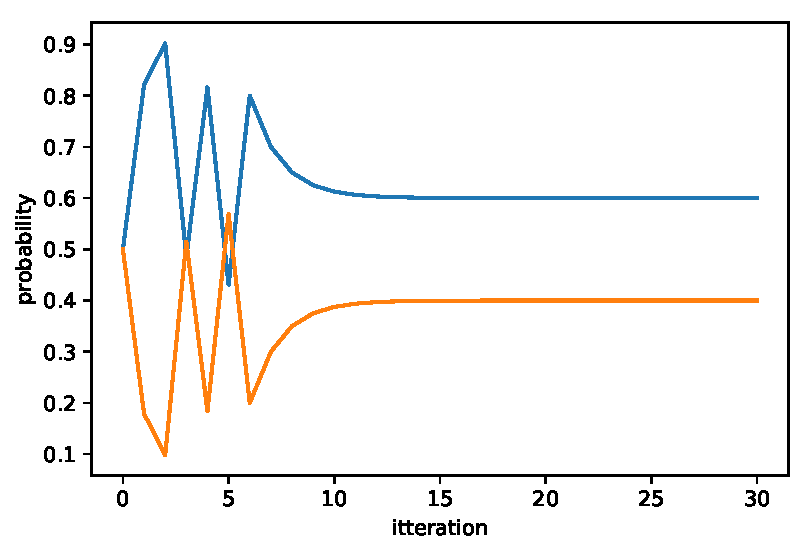
\includegraphics[width= \linewidth]{figures/hiddenMarkov_figure1_1.pdf}
\end{document}